%  pk-EFM theory paper
%  Created by Ryan P. Dwyer July 8, 2016

% %%   PREAMBLE   %%%

% PREPRINT
%\RequirePackage[displaymath,mathlines]{lineno}  % implement numbered lines
%\documentclass[aps,prl,preprint,citeautoscript,superscriptaddress,byrevtex,nofootinbib]{revtex4}
\documentclass[xcolor={dvipsnames}]{beamer}
\usetheme{Copenhagen}

% GALLEY
%\RequirePackage[displaymath,mathlines]{lineno}  % implement numbered lines -- pagewise for two-column mode
% \documentclass[10pt,aps,prl,twocolumn,galley,citeautoscript,superscriptaddress,byrevtex,nofootinbib,nobalancelastpage,floatfix]{revtex4}

% TWO COLUMN
%\RequirePackage[displaymath,mathlines,pagewise]{lineno}  % implement numbered lines -- pagewise for two-column mode
%\RequirePackage[displaymath,mathlines]{lineno}  % implement numbered lines -- pagewise for two-column mode
% \documentclass[aps,prl,twocolumn,citeautoscript,superscriptaddress,byrevtex,nofootinbib,nobalancelastpage,floatfix]{revtex4}

% PACKAGES
\usefonttheme{professionalfonts}
\usepackage{siunitx}    % package for \meter etc
\usepackage{graphicx}         % \includegraphics{}
\usepackage{amsmath}                  % \pmatrix{}, etc...
\usepackage{mathtools}
\usepackage{bm}                       % need for bold greek letters
\usepackage{mciteplus}
\usepackage{natbib}  % bibliography
%\RequirePackage{lineno}
                                    
% FONTS

% Computer Modern is the default LaTeX font.
% Uncomment one of the lines below to try another font.
% PRL actually appears to use a font closet to Times.
% \usepackage{times}     % ~not~ computer modern fonts
\usepackage{palatino}  % ~not~ computer modern fonts

% FORMATTING OPTIONS

\lefthyphenmin=3           % Fix LaTeX hyphenation
\righthyphenmin=4          % Fix LaTeX hyphenation
%\setlength{\parskip}{6pt}  % Set paragraph spacing to be easy on the eyes

\graphicspath{
{/Users/ryandwyer/Dropbox/_JAM_MS__Dwyer201607__pk_EFM_theory__figs/}
}

% COMMANDS
\newcommand{\trimcaptionspacing}{\vspace{-0.25in}}      % include in figures to decrease the text-to-figure spacing
\newcommand{\trimcaptionspacinghalf}{\vspace{-0.10in}}  % include in figures to decrease the text-to-figure spacing
\def\bibfont{\footnotesize} % Smaller font in the bibliography

% Easy text subscripts
\newcommand{\st}[1]{_\text{#1}}


% See http://tex.stackexchange.com/questions/21598/how-to-color-math-symbols
\makeatletter
\def\mathcolor#1#{\@mathcolor{#1}}
\def\@mathcolor#1#2#3{%
  \protect\leavevmode
  \begingroup
    \color#1{#2}#3%
  \endgroup
}
\makeatother

 
 
 
%Information to be included in the title page:
\title{What is the singular value decomposition?}
\author{Ryan Dwyer}
\institute{Cornell University}
\date{2016.11.07}
 
% See http://tex.stackexchange.com/a/74251 
\setbeamerfont{page number in head/foot}{size=\large}
\setbeamertemplate{footline}[frame number]

\begin{document}

\frame{\titlepage}

\begin{frame}
\frametitle{Applications of the singular value decomposition}
\begin{itemize}
    \item Approximating matrices
    \item Optimization
\end{itemize}
\end{frame}

\begin{frame}
\frametitle{Action of a matrix}
\begin{figure}
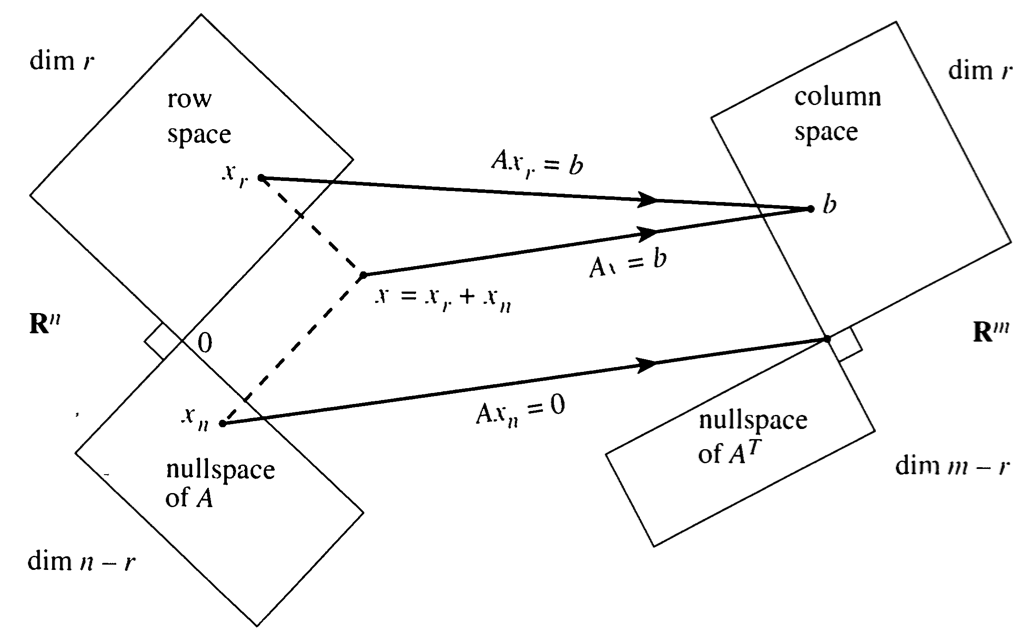
\includegraphics[width=3.75in]{figs/Strang1993nov-fig1.png}
\end{figure}
\end{frame}

\begin{frame}
\frametitle{Examples}
\begin{figure}
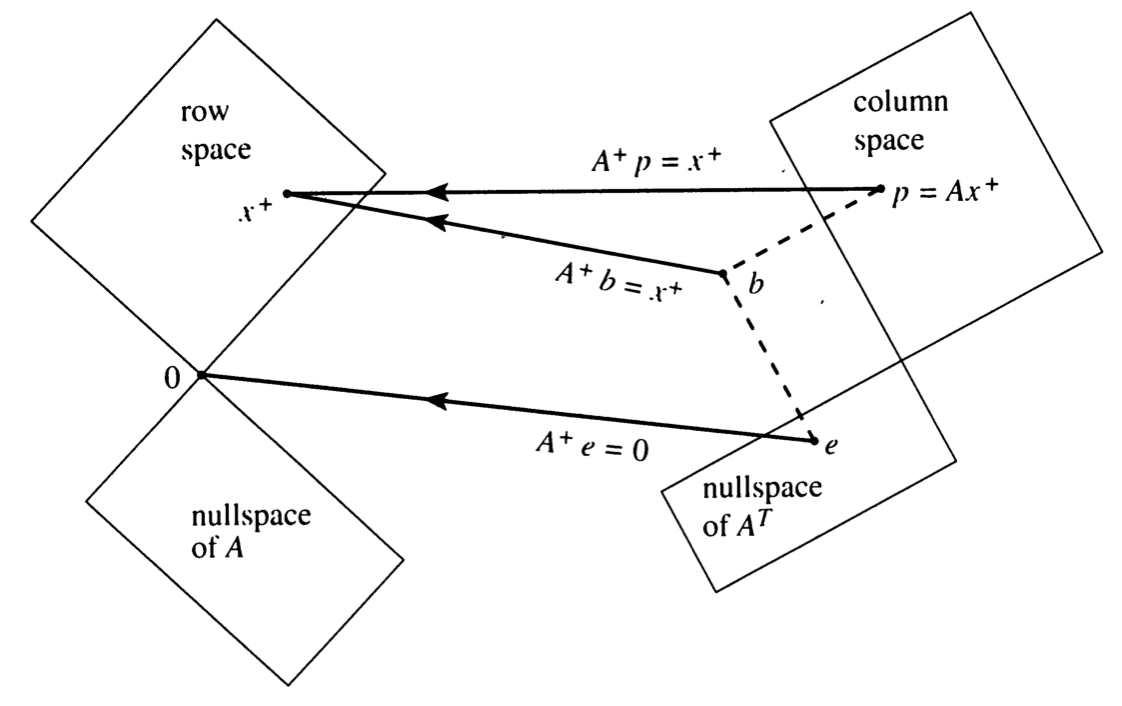
\includegraphics[width=3in]{figs/Strang1993nov-fig4.png}
\end{figure}
Linear least squares:
\begin{equation}
y = \begin{pmatrix}
-1 & 1 \\
0 & 1 \\
1 & 1 \\
\end{pmatrix}
\begin{pmatrix}
\alpha \\
\beta
\end{pmatrix}
\end{equation}
\end{frame}

\begin{frame}
\frametitle{Examples}
\begin{figure}
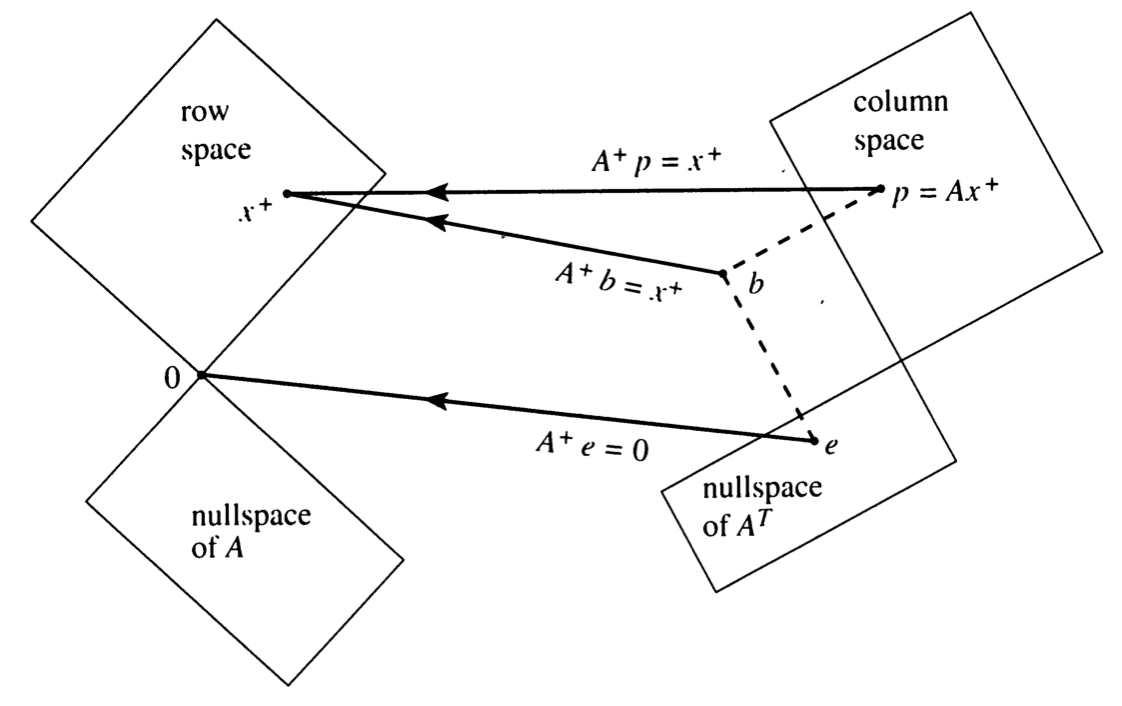
\includegraphics[width=3in]{figs/Strang1993nov-fig4.png}
\end{figure}
Linear least squares:
\begin{equation}
A = \begin{pmatrix}
-1/\sqrt{3} & -1/\sqrt{2} \\
-1/\sqrt{3} & 0 \\
-1/\sqrt{3} & 1/\sqrt{2}
\end{pmatrix}
\begin{pmatrix}
    \sqrt{3}
\end{pmatrix}
\begin{pmatrix}
\alpha \\
\beta
\end{pmatrix}
\end{equation}
\end{frame}



% =========================
% \def\bibsection{\vspace{6pt}}
% \setlength{\bibsep}{0pt}

% \bibliographystyle{bst/naturemag_jm}

% \bibliography{bib/jam99_2012-03-29_Ryan}
% \label{TheEnd}
\end{document}
